\documentclass[../thesis]{subfiles}
\graphicspath{{\subfix{../figures/}}}
\begin{document}
\chapter{Introduction}

\lettrine[lines=3]{\textcolor{Maroon}{L}}{anguage} Servers have become an increasingly popular way to offer "code smarts," such as code autocomplete or the highlighting of errors.
However, even though the Language Server Protocol has been written to be broadly compatible with any development tool, in practice, it has only been used for traditional IDEs and editors instead of more modern and unconventional approaches like code cities.
I am of the opinion that code cities can benefit from making use of this protocol, so the core focus of this master's thesis is going to be combining it with code cities, specifically SEE.

The main novel contribution will be a way of creating code cities using only information provided by the \glsentrylong{lsp}, while additional contributions consist of the integration of \glsentrylong{lsp}-based functionality into code cities as well as their integration into SEE's code windows.
Finally, the penultimate \cref{ch:evaluation} describes a controlled experiment (with $n=\participants$ participants) in which code cities are compared to traditional IDEs via a user study---this serves as an evaluation for this thesis and for code cities as IDE replacements in general.

In this chapter, apart from explaining some formatting semantics, we will examine the motivation and basics behind each of the central concepts (\ie, code cities, the \glsentrylong{lsp}, and the integration of the two), name the goals and research question of the thesis, and finally describe the structure of upcoming chapters.

\section{Format}

This document uses many technical terms that not every reader may know.
To remedy this, starting from the next section, whenever a technical term or acronym appears for the first time, it will be printed in \emph{\textcolor{Maroon}{this color}}, and an explanation of that term will appear in a footnote of the same color.
Terms that are already explained in the text itself will not receive such a footnote.
These terms and acronyms are collected within the glossaries in \cref{main,abbreviations}---all mentions of such terms also link (in the digital version of this thesis, at least) to the corresponding part of the glossary.
Hence, if you come across a technical term or abbreviation you are not familiar with, simply try clicking on it.
In total, the following colors are used to convey specific meanings:
\begin{itemize}
	\item \textbf{\textcolor{Maroon}{Maroon}} for the introduction of a glossary term or acronym,
	\item \textbf{\textcolor{Fuchsia}{Fuchsia}} for internal links (\eg, to other sections),
	\item \textbf{\textcolor{Blue}{Blue}} for external links (\eg, to web pages),
	\item \textbf{\textcolor{ForestGreen}{Green}} for cited literature, and
	\item \textbf{\textcolor{Cyan}{Cyan}} for references to attached files (see \cref{file}).
\end{itemize}

\section{Motivation}
As mentioned at the beginning of this chapter, this master's thesis is about \emph{integrating} the \emph{Language Server Protocol} into \emph{Code Cities}.
I will motivate each of these italicized central points individually in the following sections.
Note that these will get more thorough explanations in \cref{ch:concepts}.

\subsection{Code Cities \& SEE}\label{subsec:see}
Visualization in general often helps facilitate the understanding of complex systems by representing them with a simplified visual model.
This can be especially useful in the area of software engineering, where it is often hard to get an intuitive overview of large software systems when only equipped with standard tools, like \glspl{ide}.
One such software visualization---called \SEE{}---is being developed at the University of Bremen and will be introduced in the next section.

\SEE{} is an interactive software visualization tool using the \gls*{city} metaphor in 3D, developed in the {Unity} game engine.
It features collaborative "multiplayer" functionality across multiple platforms\footnote{
	Notably, besides usual desktop and touchscreen-based environments, virtual reality (\eg, via the \emph{Valve Index}) is supported as well.
}, allowing multiple participants to view and interact with the same \gls*{city} together.

\begin{figure}[hbtp]
	\centering
	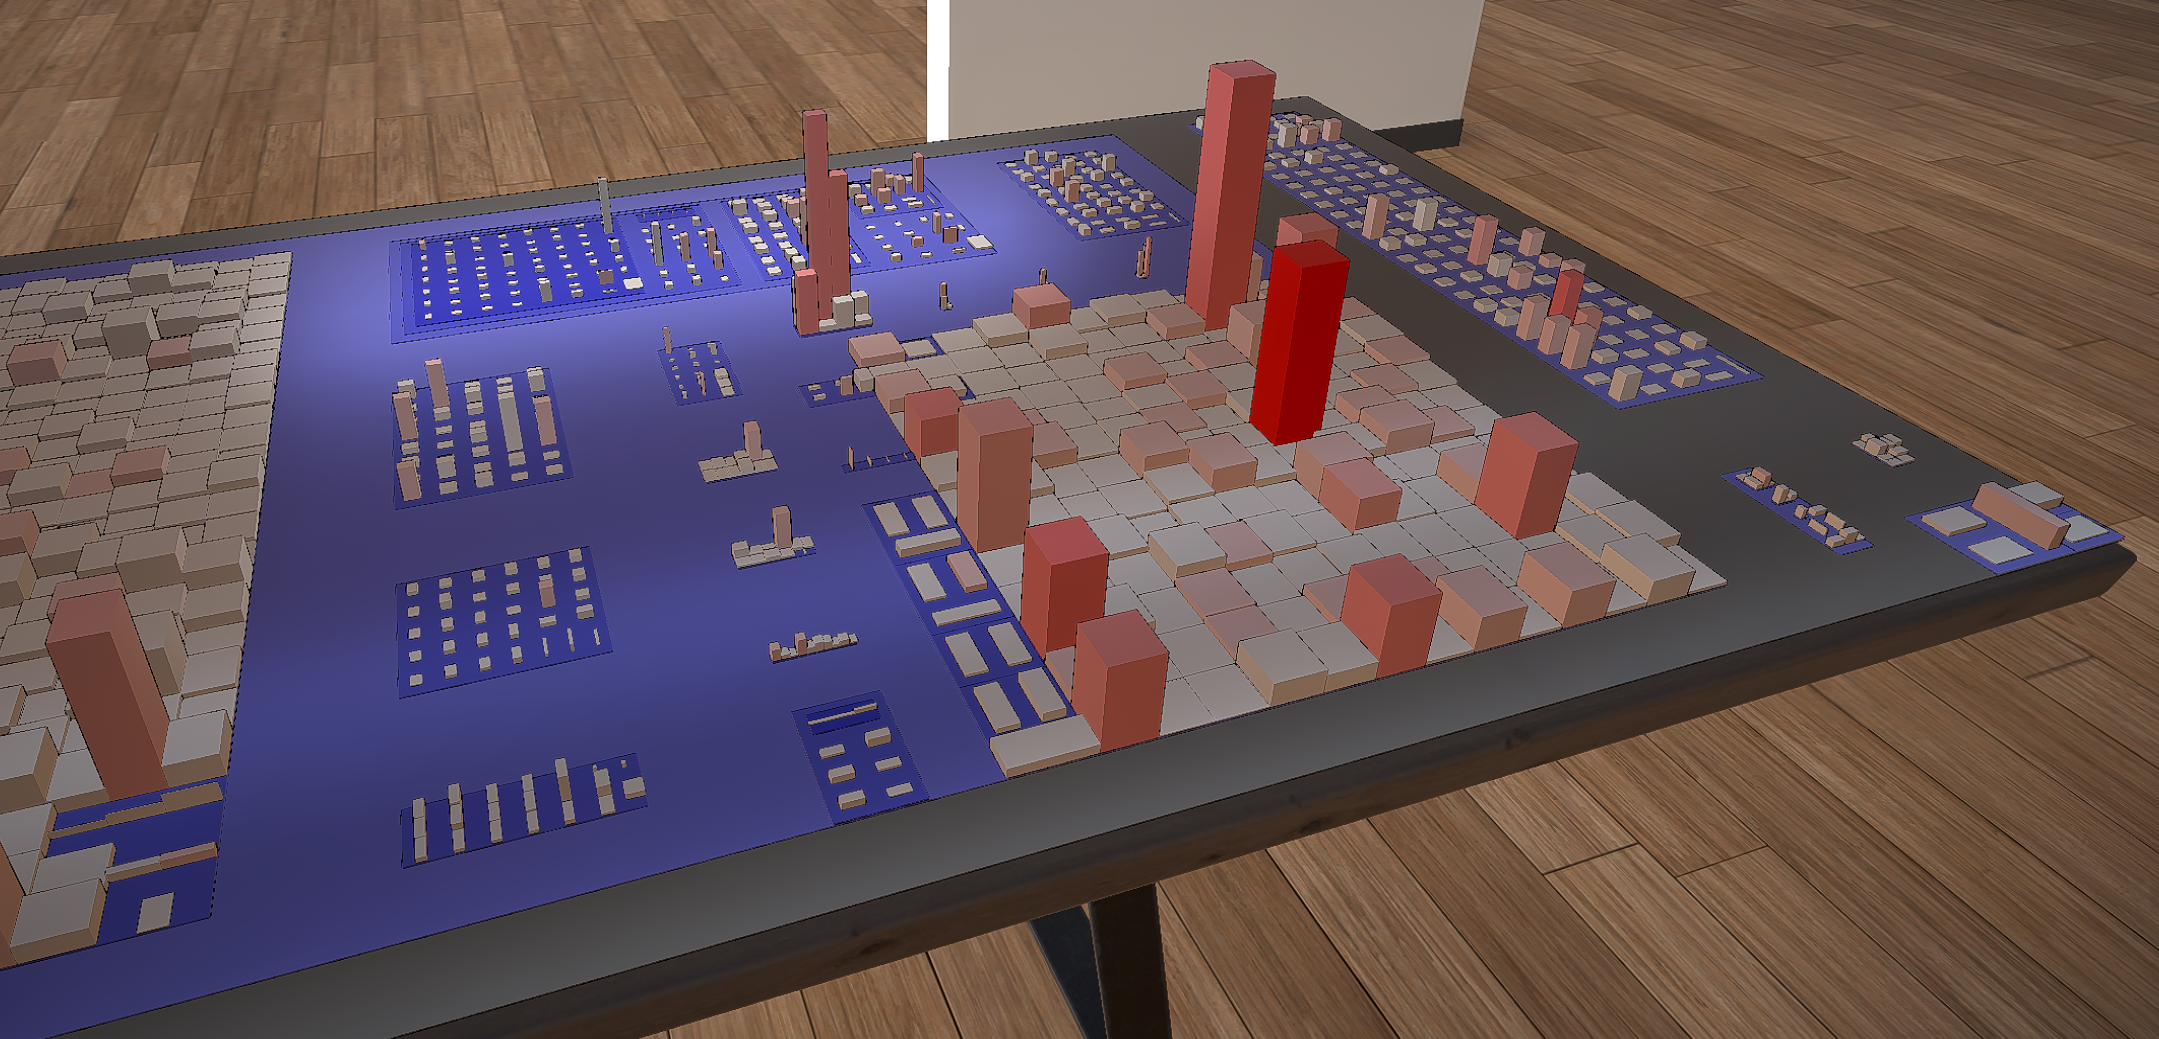
\includegraphics[width=\textwidth]{SEE_screenshot}
	\caption{A \gls{city} visualized in \SEE{}.}\label{fig:city}
\end{figure}

In the \gls{city} metaphor, software components are visualized as buildings within a city.
Various metrics from the original software can then be represented by different visual properties of each building---for example, the \gls{loc} within a file might correlate to the height of the corresponding building.
Relationships between software components, such as where components are referenced, are instead represented by edges drawn between the respective buildings.
The exception to this are part-of relations, that is, relations that describe which component belongs to which other component.
These are instead visualized in \SEE{} by buildings being nested within their corresponding "parent" building.
In this way, the data model of \SEE{} can be represented as a graph in which the software components are the nodes and the relationships are the edges.

For example, in \cref{fig:city}, we can see the source code of the SpotBugs project~\cite{spotbugs} rendered as a \gls{city}.
A few very tall buildings---indicating that the respective component is very big and that a refactoring into smaller pieces may be in order---immediately jump out.
Additionally, this visualization also makes the number of methods readily apparent:
the redder a node, the higher its method count.
\Cref{fig:edges} instead visualizes the modeled architecture of a very small system, as compared to a city "empirically" generated by an implementation like in the previous example.
Here, we can also see yellow edges between the components, in this case representing desired references that should be present between components.

\begin{figure}[hbtp]
	\begin{center}
		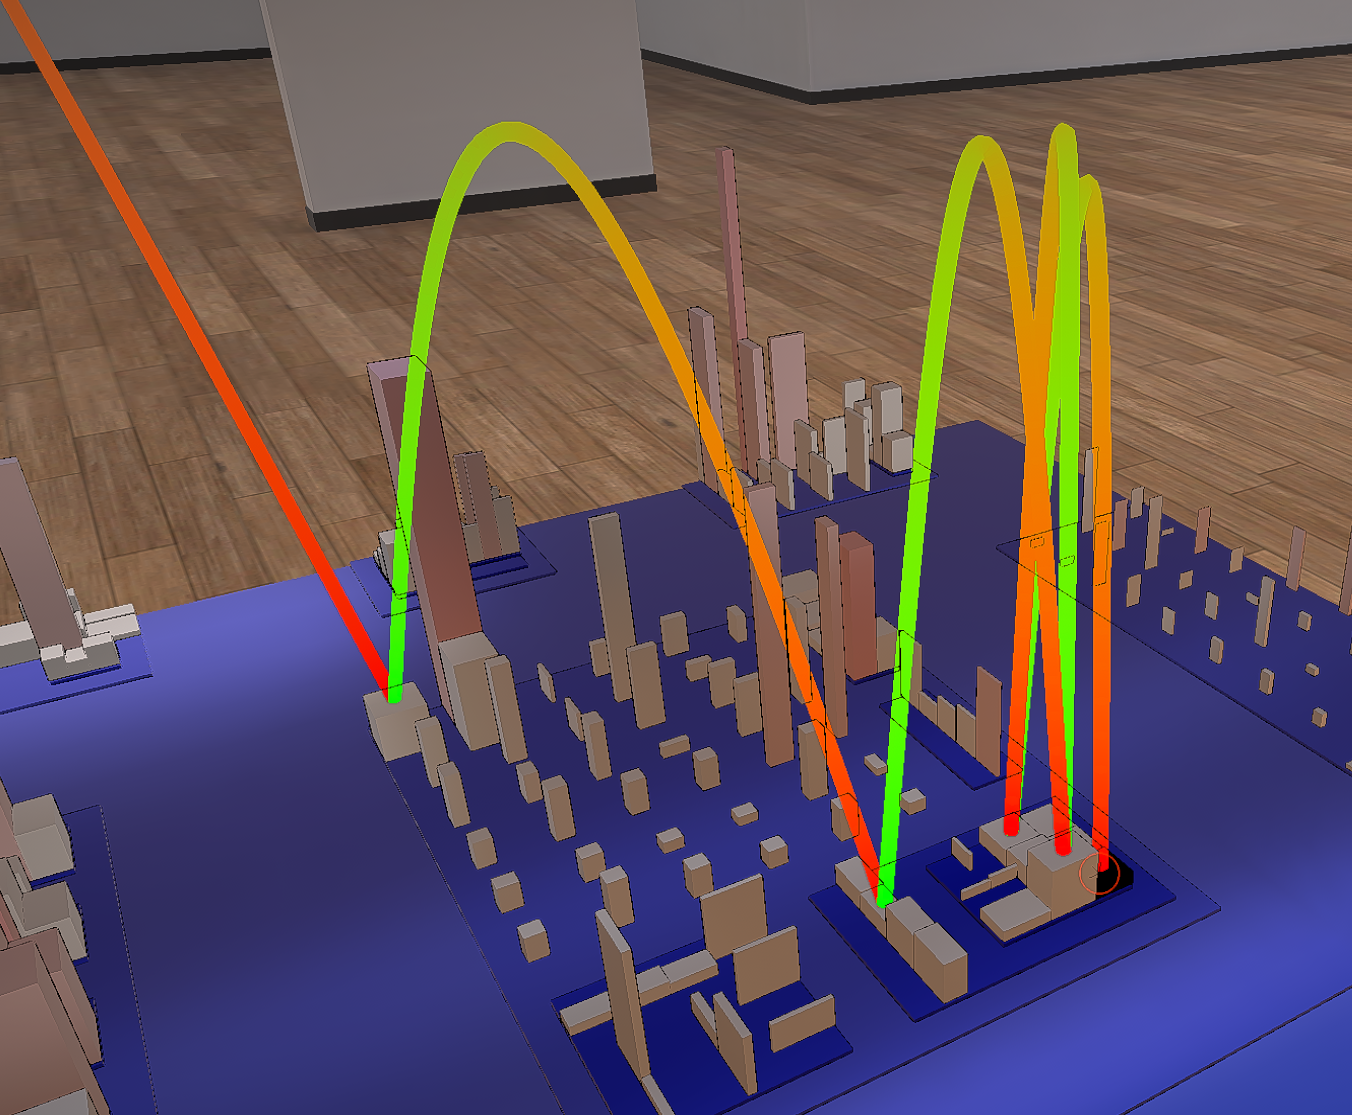
\includegraphics[width=0.7\textwidth]{SEEEdges}
	\end{center}
	\caption{An example of what edges can look like in \SEE{}.}\label{fig:edges}
\end{figure}

\subsection{Language Server Protocol}\label{subsec:lsp}

As stated on its website:
\begin{displayquote}[\cite{lsp}]
	Adding features like auto complete, go to definition, or documentation on hover for a programming language takes significant effort. Traditionally[,] this work had to be repeated for each development tool, as each tool provides different APIs for implementing the same feature.

	A \gls*{ls} is meant to provide the language-specific smarts and communicate with development tools over a protocol that enables inter-process communication.

	The idea behind the \gls*{lsp} is to standardize the protocol for how such servers and development tools communicate. This way, a single \gls{ls} can be re-used in multiple development tools, which in turn can support multiple languages with minimal effort.
\end{displayquote}

\noindent{}Since \gls{lsp}\footnote{%
	Note that I will often refer to the \glsentrylong{lsp} as just "\gls{lsp}" instead of "the LSP" (\eg, "\glspl{ide} use \gls{lsp}") from now on, as this is how the specification~\cite{lsp} does it as well.
} is a central component of my master's thesis, I have created a diagram in \cref{fig:lsp} in the hope to strengthen intuitions around the motivation and use of the protocol.
While the \gls{lsp} specification has originally been created by Microsoft, it is by now an open-source project\footnote{
	Available at \web{https://github.com/Microsoft/language-server-protocol}{2024-09-11}.
}, where changes can be actively proposed using issues or pull requests.
Apart from the specification itself, a great number of open-source implementations of \glspl{ls} for all kinds of programming languages from Ada to Zig exist.
A partial overview of available implementations is listed at \web{https://microsoft.github.io/language-server-protocol/implementors/servers/}{2024-09-11}.

\begin{figure}[hbtp]
	\begin{center}
		\subcaptionbox{\gls{ide} development without \gls{lsp}.\label{fig:lspwithout}}{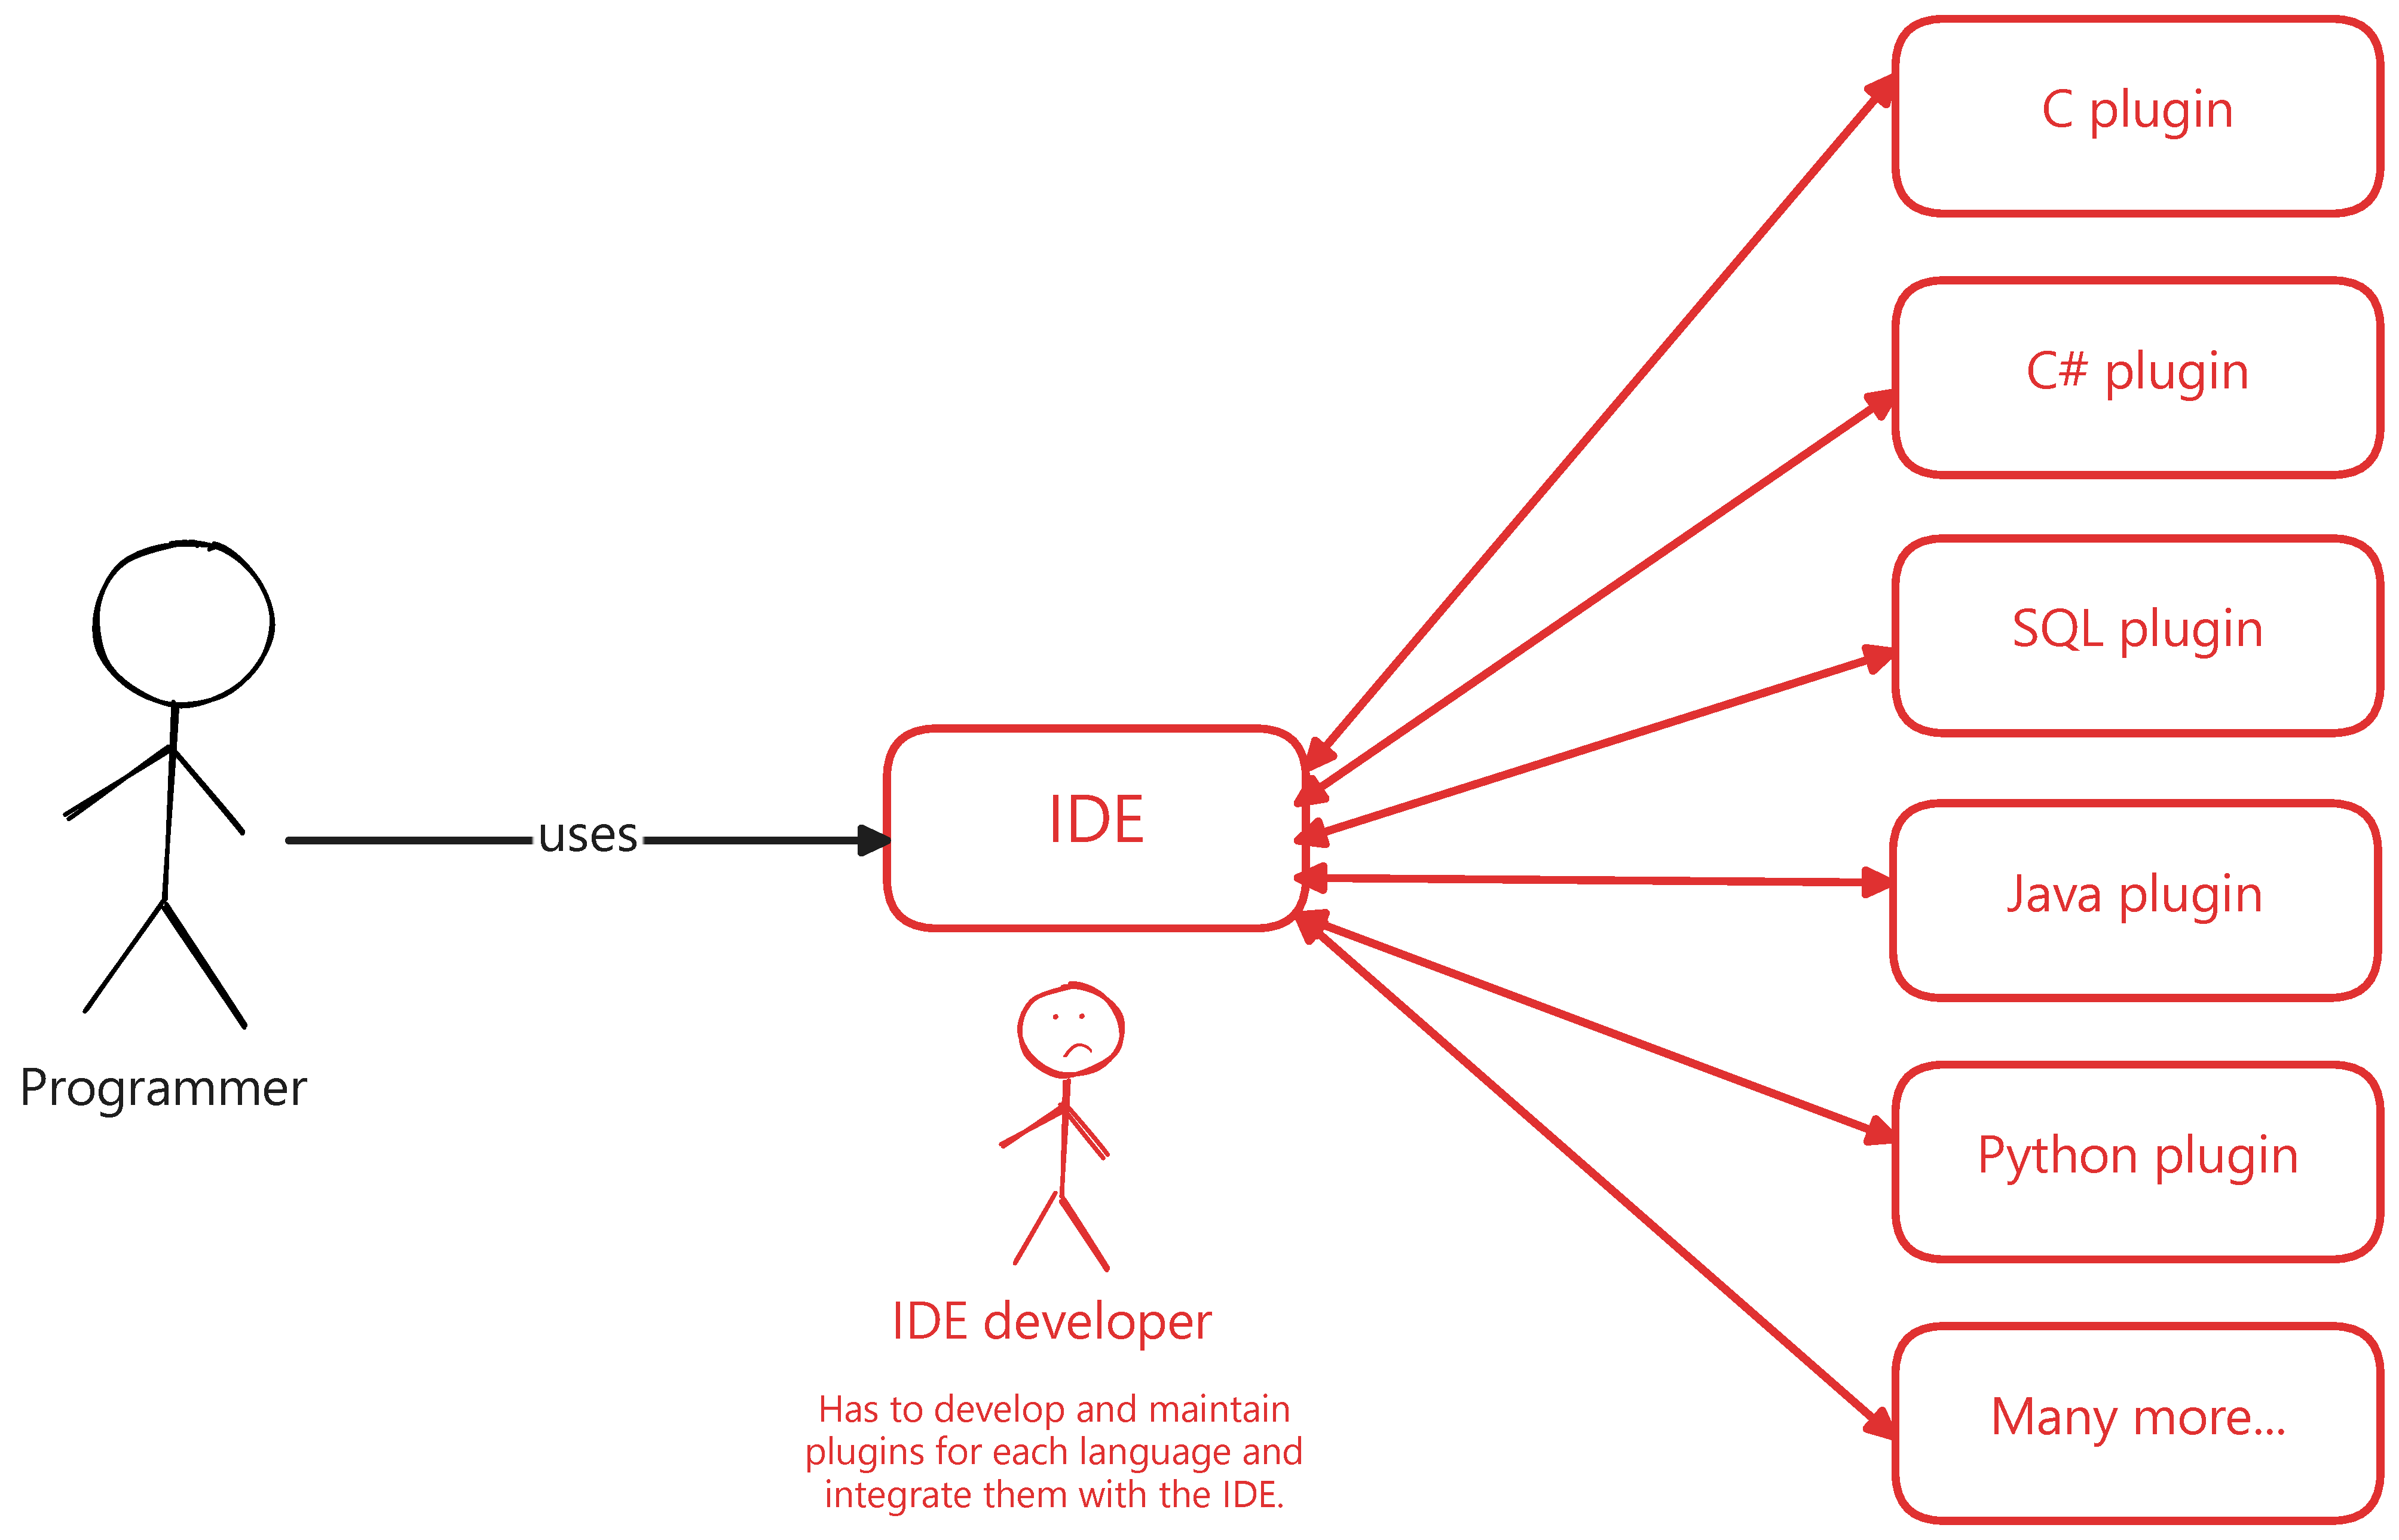
\includegraphics[width=0.95\textwidth]{../figures/overview_lsp_without_lsp}}
		\subcaptionbox{\gls{ide} development with \gls{lsp}.\label{fig:lspwith}}{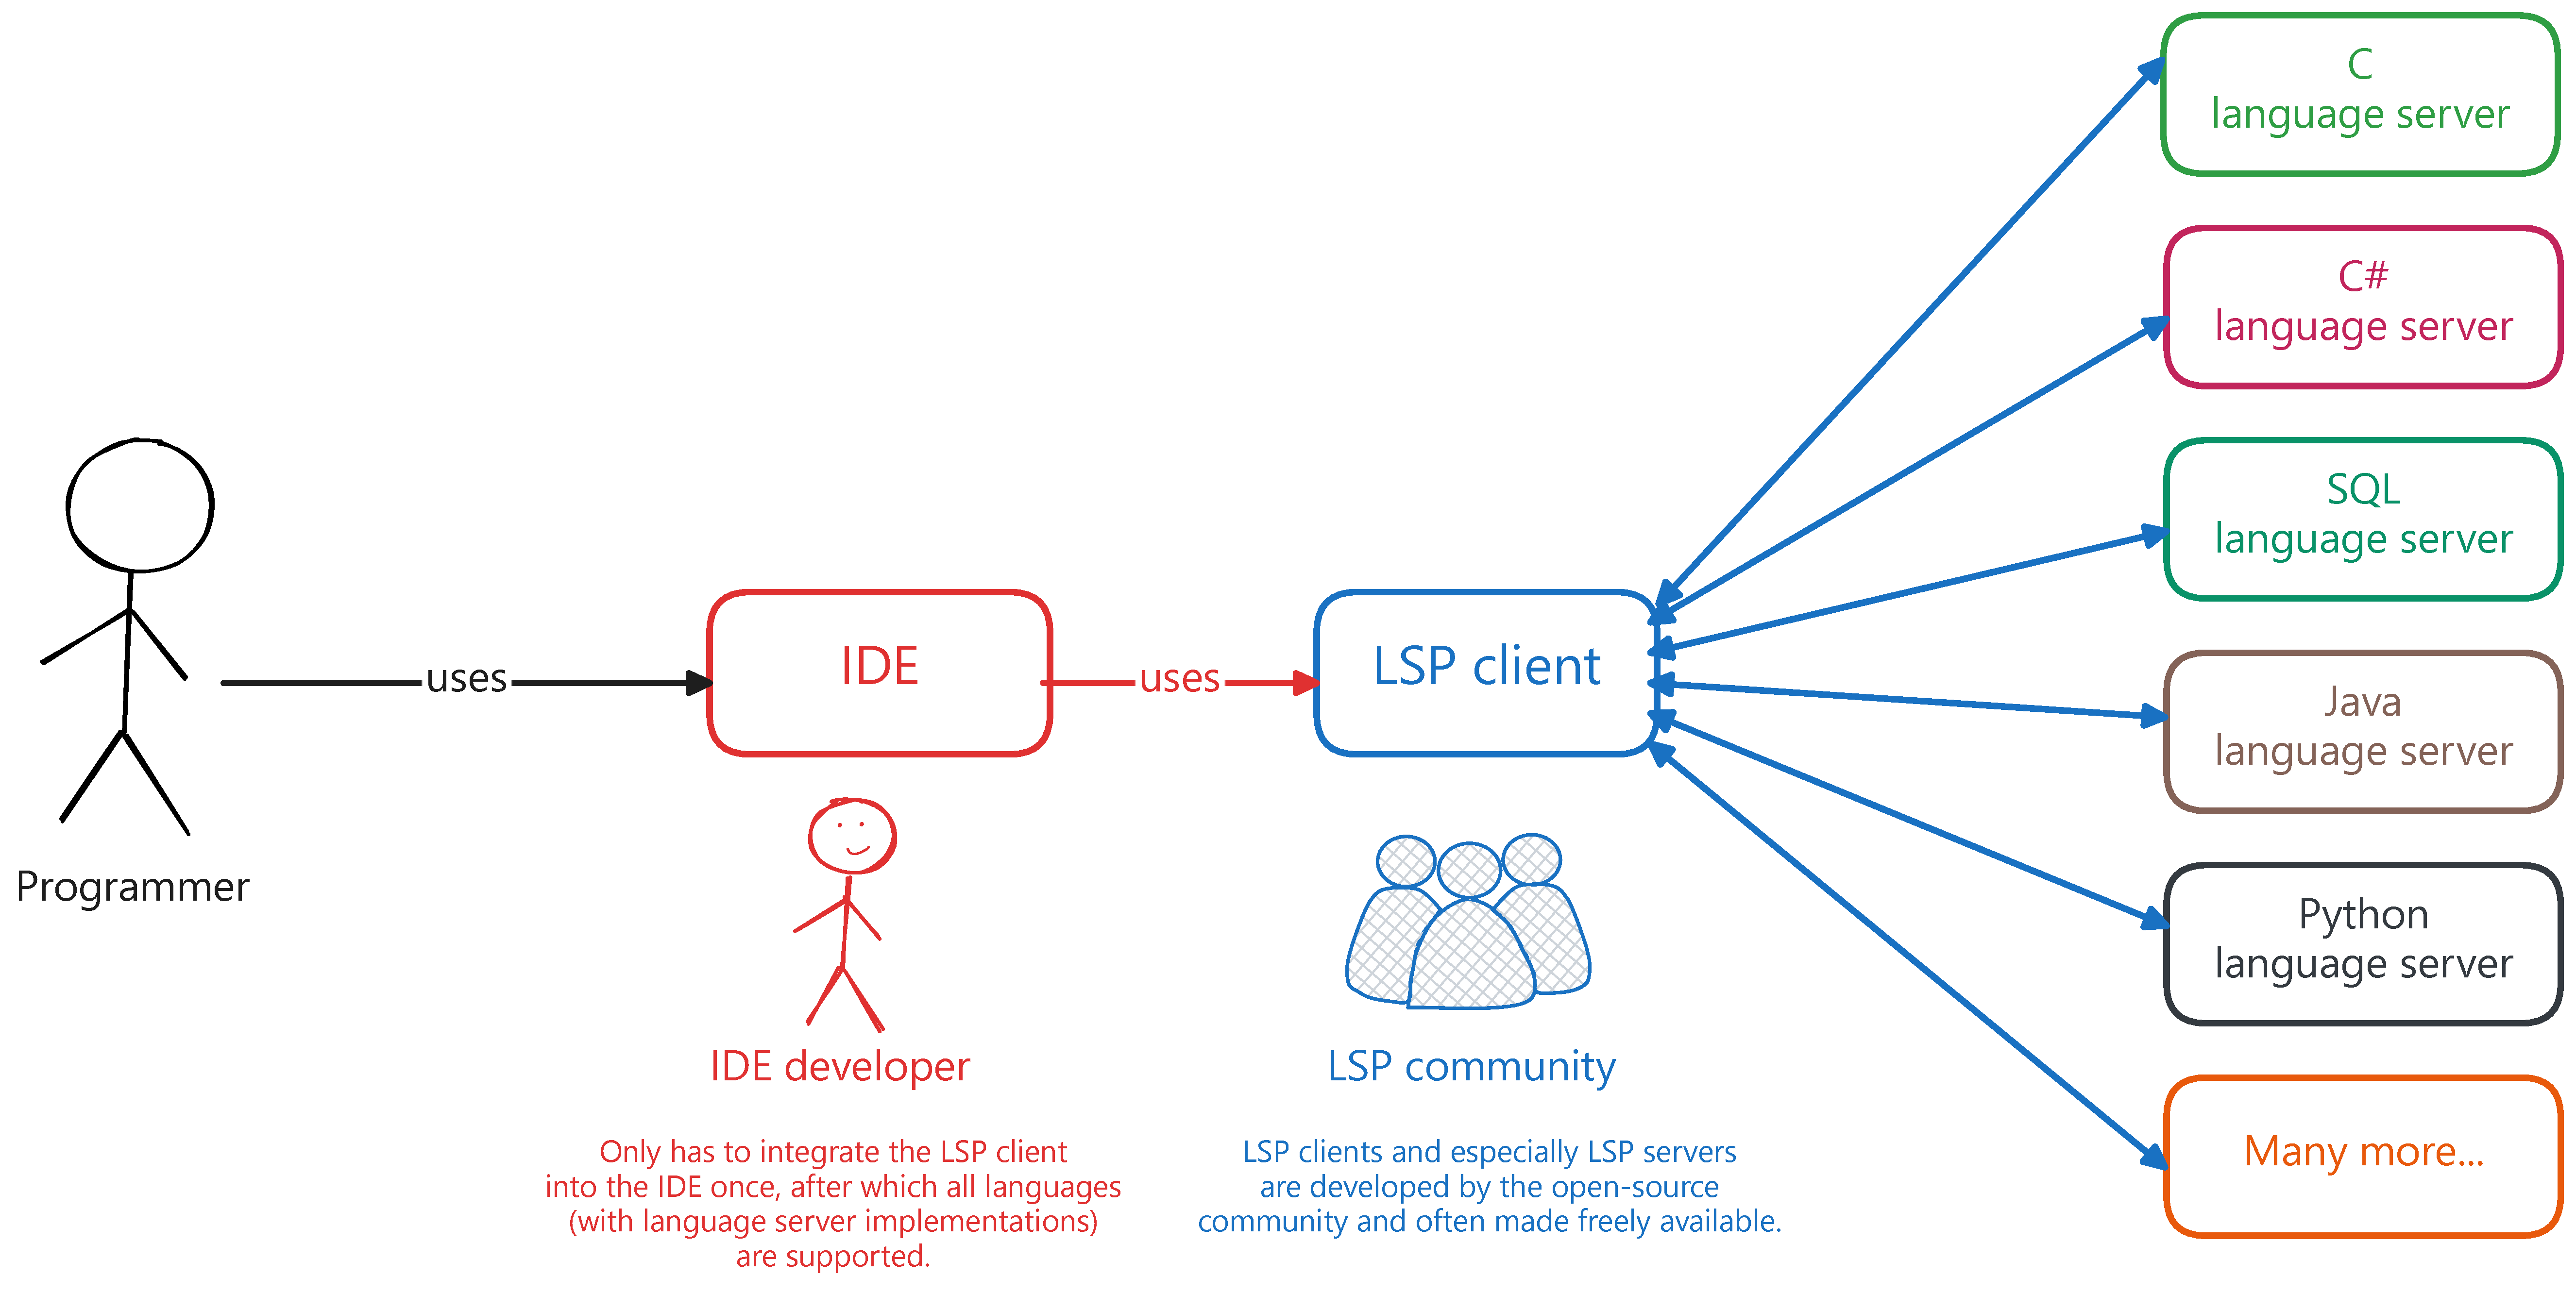
\includegraphics[width=0.95\textwidth]{../figures/overview_lsp_with_lsp}}
	\end{center}
	\caption{An illustration of how \gls{lsp} can help simplify \gls{ide} development.}\label{fig:lsp}
\end{figure}

The protocol introduces the concept of so-called \glspl*{capability}, which define a specific set of features a given \gls{ls} (and \gls{lc}) support.
These include navigational features, like the ability to jump to a variable's declaration, and editing-related features, such as autocomplete.
To give a specific example of what an \gls{lsp} \gls{capability} might look like in practice, the \tt{texlab}~\cite{forster2025} \gls{ls} for \LaTeX{}---which I am using while writing this document---provides a list of available packages when one starts typing text after "\mintinline{LaTeX}+\usepackage{+".
Additionally, for the currently hovered package, a short description of it is displayed.
A screenshot of this behavior within the Neovim editor is provided in \cref{fig:mwe}.

\begin{figure}
	\begin{center}
		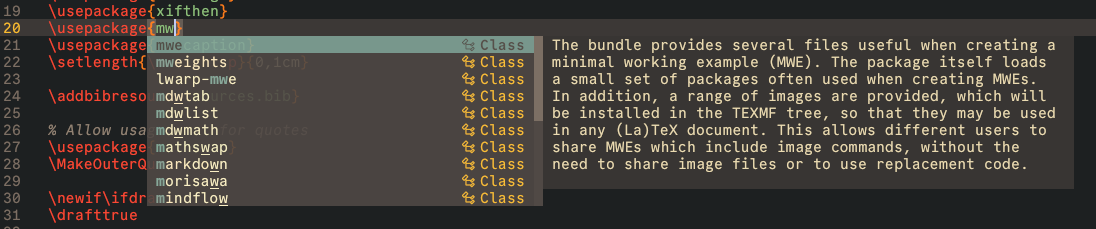
\includegraphics[width=0.95\textwidth]{../figures/mwe}
	\end{center}
	\caption[An example of the \texttt{texlab} language server running in Neovim.]{An example of the \tt{texlab} \gls{ls} running in Neovim.}\label{fig:mwe}
\end{figure}

The counterparts to \glspl{ls} are the \glspl{lc}:
These are the IDEs and editors that incorporate the \gls{ls} into themselves.
Examples for IDEs that support acting as a \gls{lc} in the \gls{lsp} context include \emph{Eclipse, Emacs, IntelliJ, Vim}, and \emph{\gls{vscode}}.

\subsection{Integration}\label{subsec:integration}
Currently, \glspl{city} in \SEE{} are rendered by reading in pre-made \gls{gxl} files, which can be created by the proprietary Axivion Suite.
This approach has the disadvantage of only supporting languages supported by the Axivion Suite, as well as making regenerating cities (\eg, if the source code changed) fairly cumbersome.
Another current shortcoming of \SEE{} is that information about the source code available to the user is limited when compared to an \gls{ide}---for example, quickly displaying documentation for a given component by hovering over it is not supported.
This is where the Language Server Protocol can help.


% SEE as it exists right now has two shortcomings relevant for this thesis when compared to a traditional IDE.
% For example:
% - uses GXL files as mentioned before, which are generated using proprietary Axivion Suite. Hence support is determined by support of Axivion Suite, which is languages XYZ.
% - Code Windows, the closest equivalent to an IDE in SEE, do not support features programmers are used to from other IDEs, such as
%    - Navigation
%    - Diagnostics (mention code smells via dashboard, link bach thesis)
%    - Show references
%    - Show documentation/signature/other info on hover
%    => note here that editing is not on the roadmap anyway, link mbleck's bachelor thesis.
%
% LSP is a good fit to solve all of these problems.
% => Describe how
% => Describe breadth of \gls{ls} implementations
% => Maybe some numbers on how far it's used
% => Do some research on Google Scholar etc for LSP papers

\begin{figure}
	\begin{center}
		\subcaptionbox{\SEE{} as it exists right now. The analyzers on the right are developed by Axivion.}{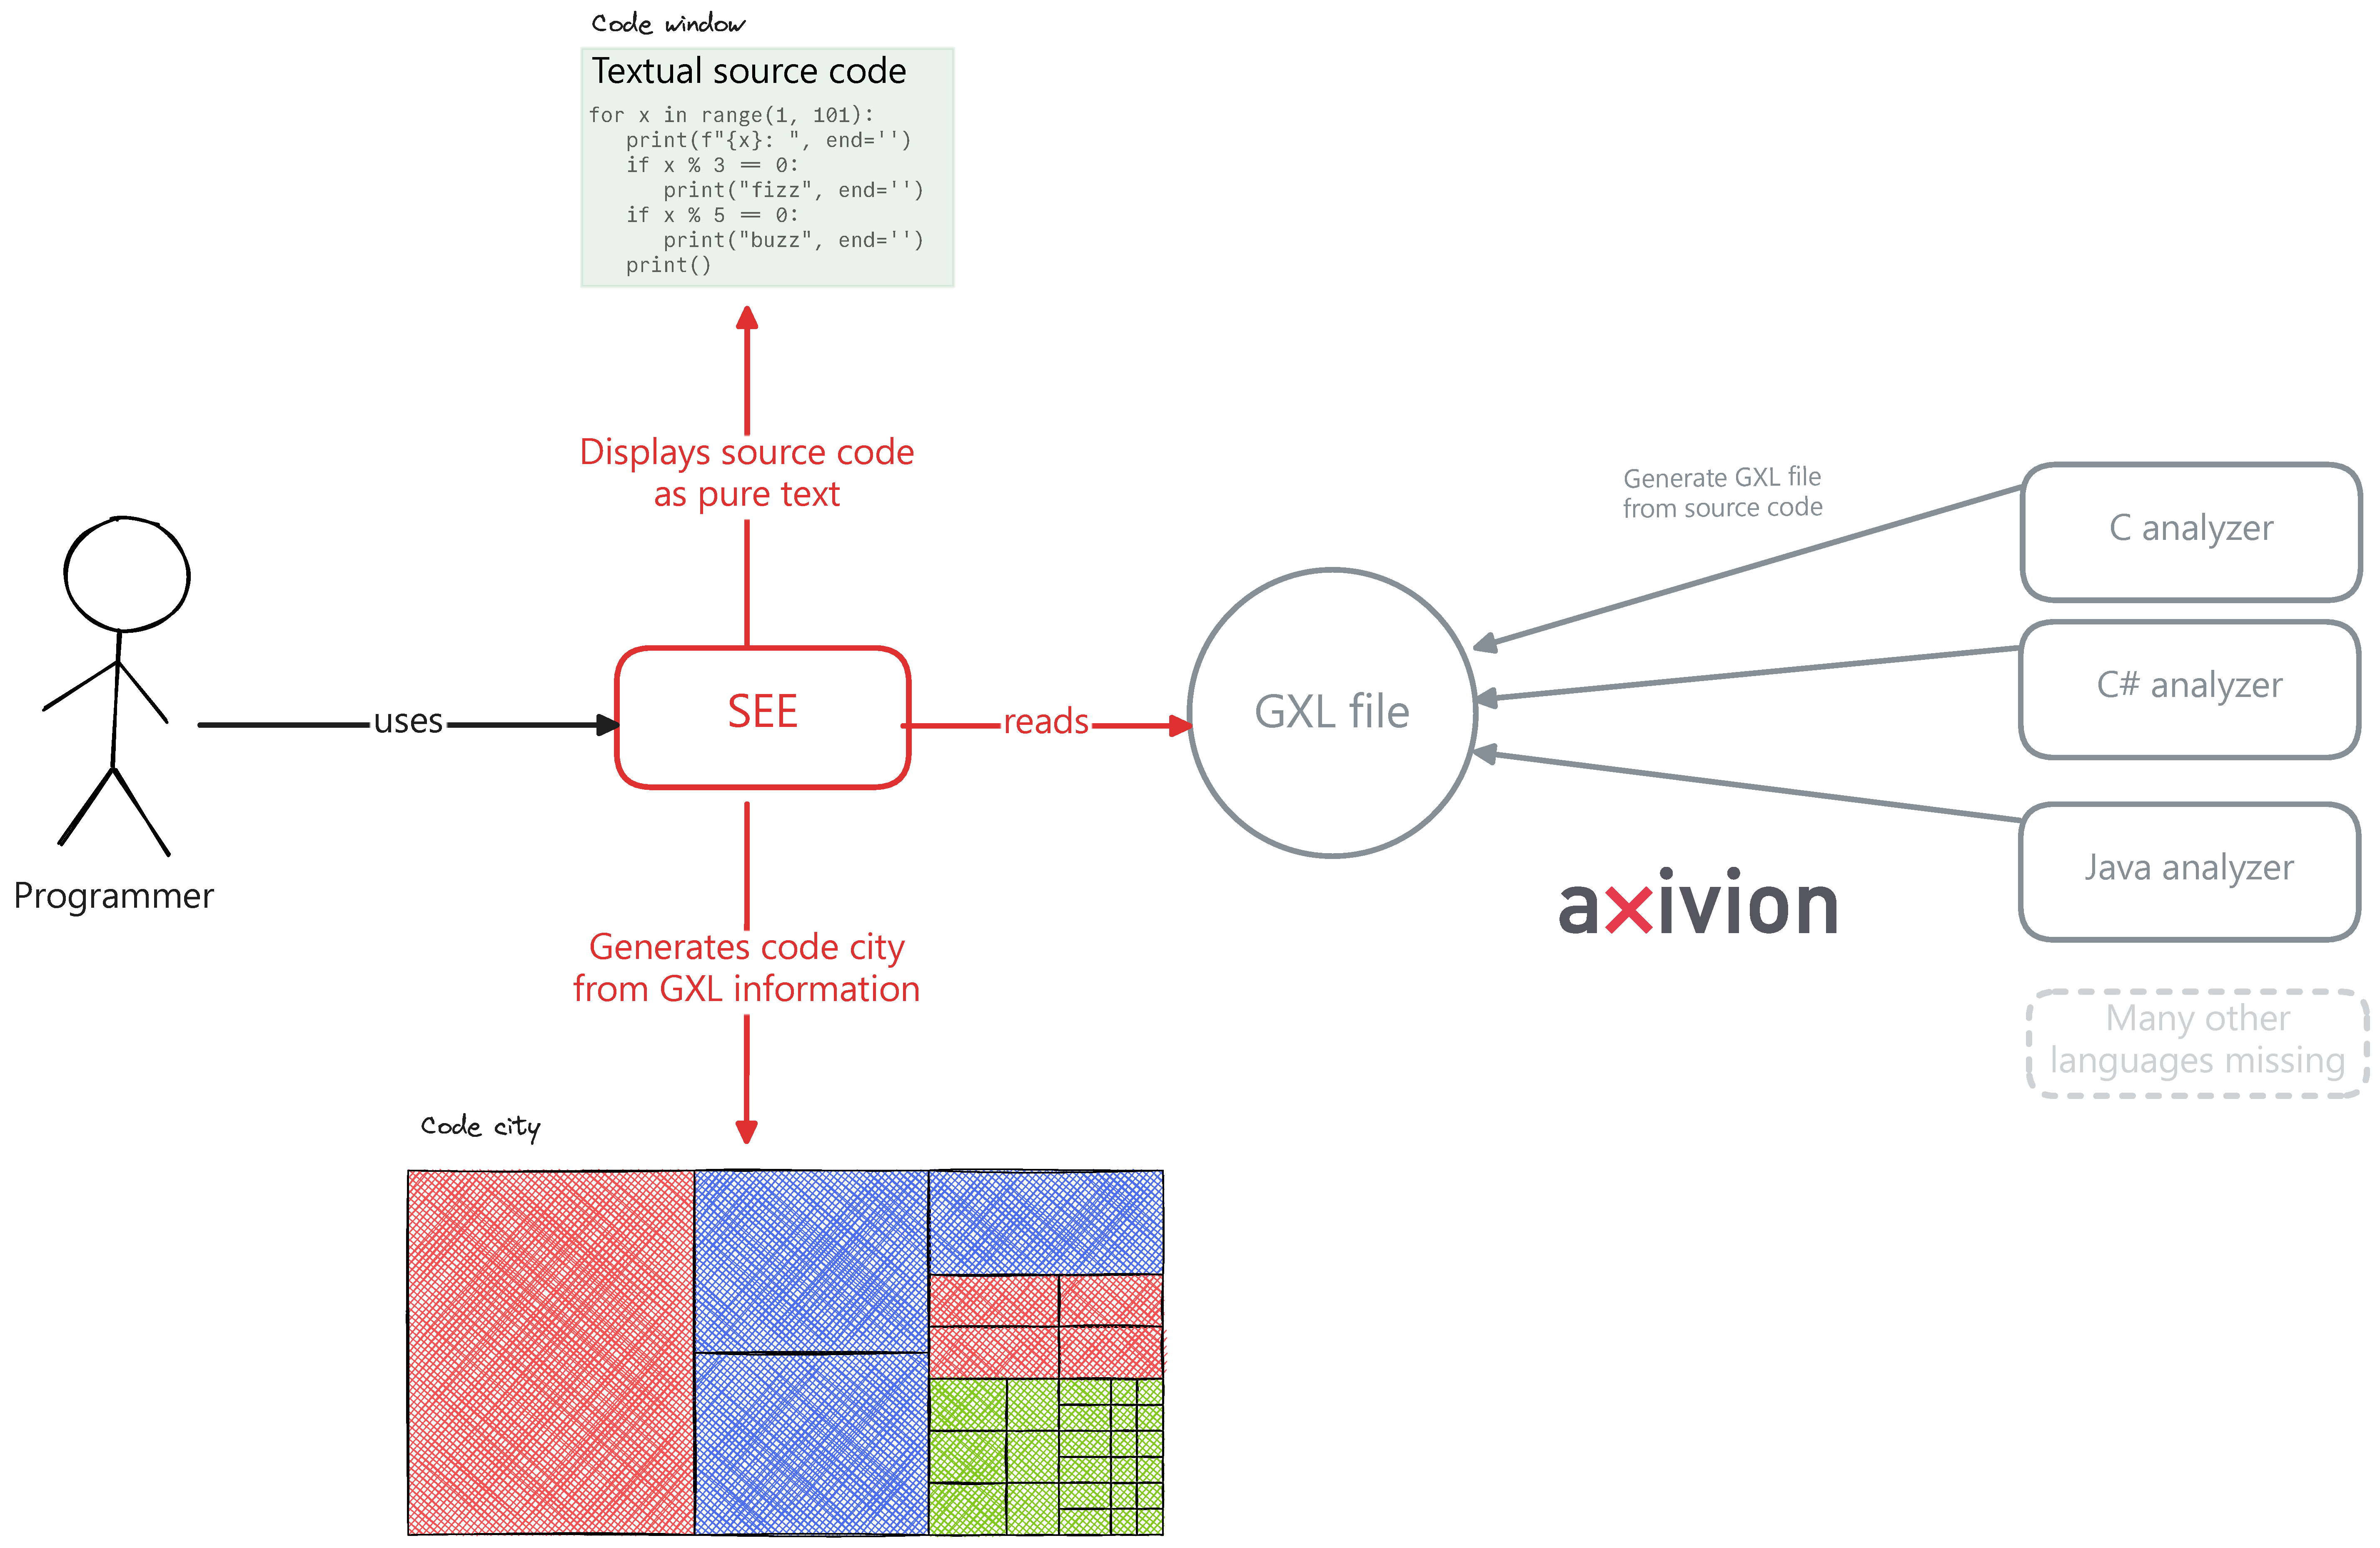
\includegraphics[width=0.95\textwidth]{../figures/overview_see_without_lsp}}
		\subcaptionbox{\SEE{} with implemented \gls{lsp} integration. The \glspl{ls} on the right are mostly developed by the open-source community.}{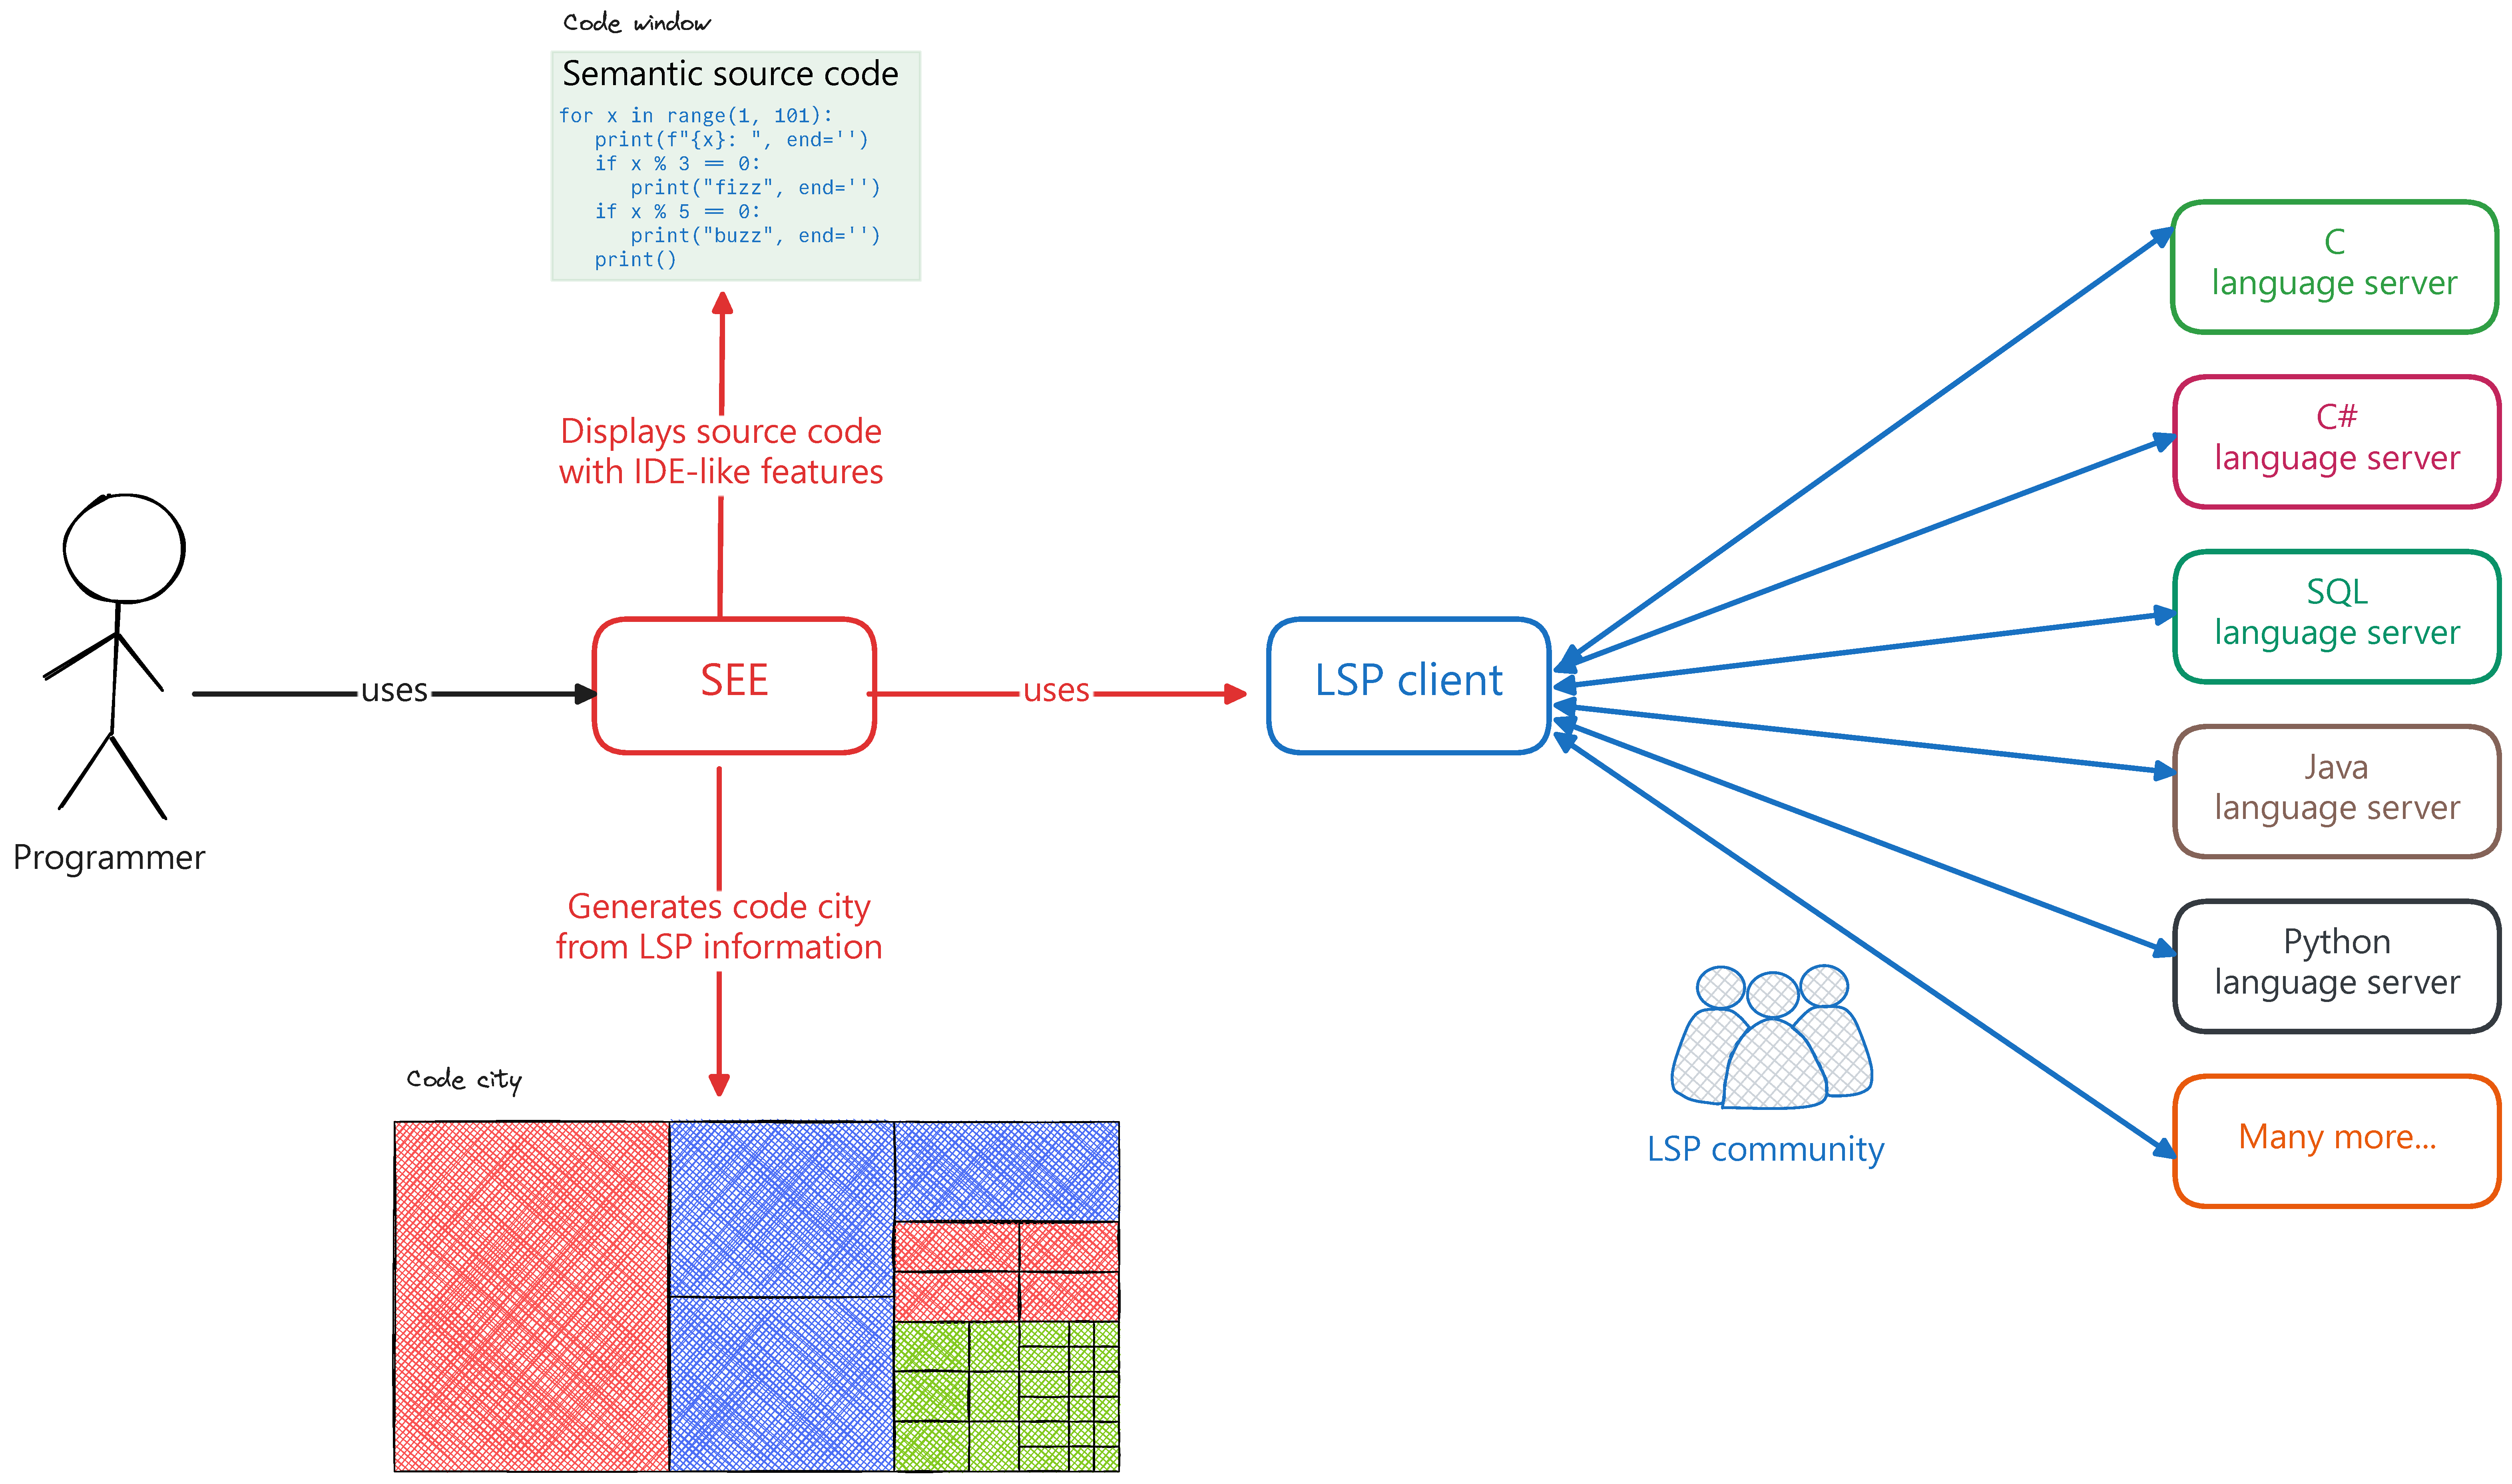
\includegraphics[width=0.95\textwidth]{../figures/overview_see_with_lsp}}
	\end{center}
	\caption{A simplified illustration of how \SEE{} currently gains and uses information about software projects, and how the integration of \gls{lsp} would change that.}\label{fig:seeplan}
\end{figure}

\fxwarning{Convert sketches here into proper TikZ diagrams}

\section{Goals \& Research Questions}\label{sec:goals}
The goal of this master's thesis---as outlined in \cref{subsec:integration}---is to integrate the \glsentrylong{lsp} into \SEE{} by making it a \gls{lc}, then evaluate this implementation by comparing it with traditional \glspl{ide} in a user study.
To this end, the main contribution is a way of generating \glspl{city} using the \gls{ls}, where all the information obtainable by relevant \gls{lsp} \glspl{capability} should be manifested\footnote{
	Since there is a lot of diverse data available via \gls{lsp}, it makes sense to only immediately display the most pertinent information and make the rest of it available upon request within \SEE{}'s user interface.
} in the city in a suitable way.
This is an unintended (or at the very least, unusual) use of \gls{lsp} and may require some experimentation.

\begin{wrapfigure}{L}{0.6\textwidth}
	\centering
	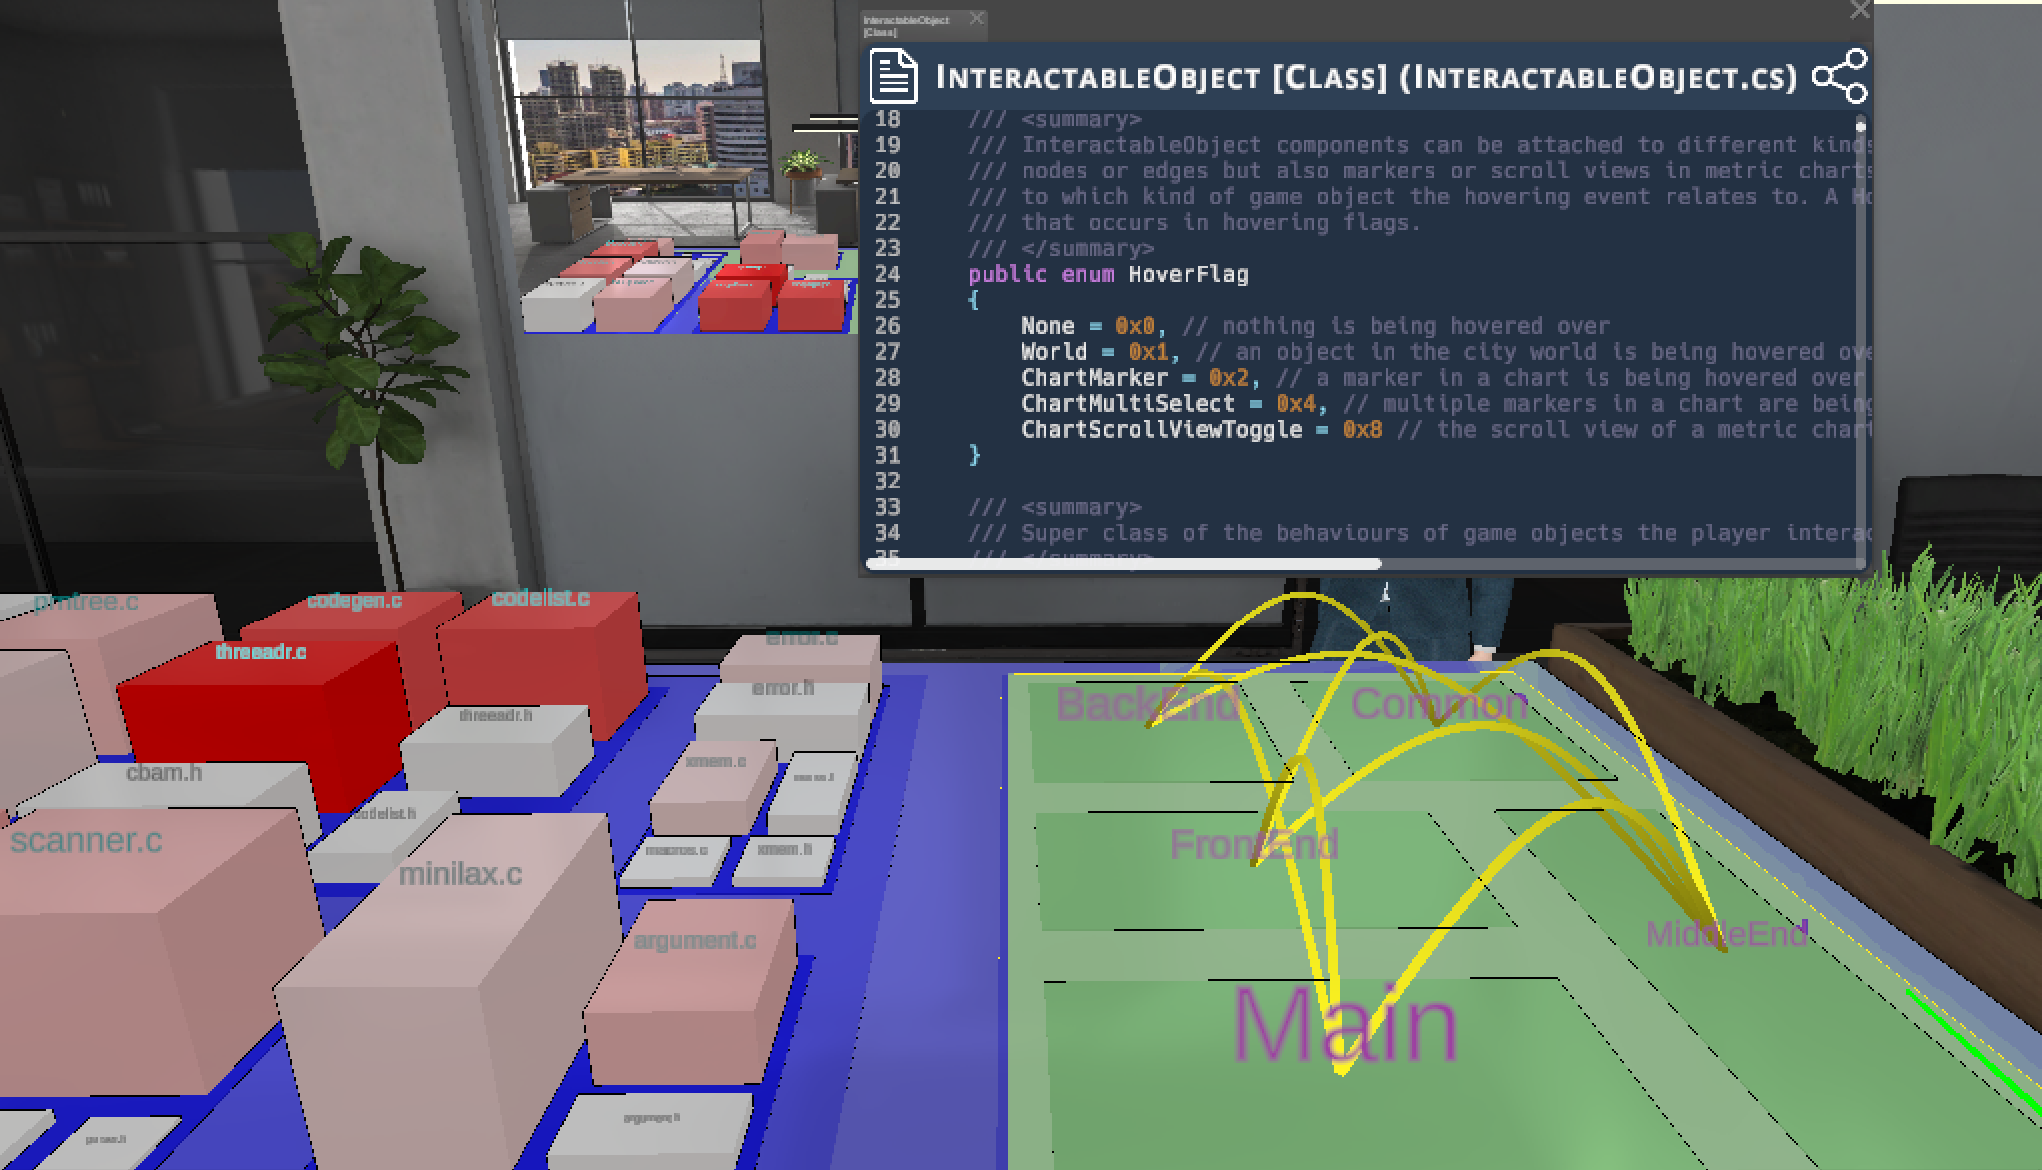
\includegraphics[width=0.6\textwidth,trim={30.5cm 22cm 6cm 0},clip]{../figures/SEE_readme}
	\caption{A code window.}\label{fig:window}
\end{wrapfigure}

Apart from the \glspl{city}, \SEE{} also provides the so-called \glspl*{window}, in which the source code of a specific component can be viewed in a similar way as in an \gls{ide}.
This can be seen in \cref{fig:window}.
An additional goal of this master's thesis is to enhance the functionality of the \glspl{window} by implementing more \gls{ide}-like behavior into it (\eg, allowing users to go to a variable's declaration, or displaying diagnostics inline) using the \gls{ls}.

It should be noted that any \gls{lsp} capabilities which involve modifying the underlying software project is out of scope for this master's thesis.
Rewriting the \glspl{window} to be editable (in a way that distributes the edits over the network) is complex enough to warrant its own thesis~\cite[see also][]{moritz}, not even taking into account that this would also more than double the number of \glspl{capability} that would then become useful to implement.
As such, only \glspl{capability} that are "read-only" (\ie, that do not modify the source code or project structure in any way) will be implemented as part of the thesis.
Consult \cref{subsec:capabilities} for a full list of \gls{lsp} capabilities implemented as part of this thesis.

Additionally, I will not implement the C\# interface to the \gls{lsp} (\ie, translating between C\# method calls and \glspl{jrpc}).
There already exist well-made interfaces for this purpose\footnote{
	Such as OmniSharp's implementation of \gls{lsp} in C\#~\cite{csharplanguageserverprotocol2025}, which I will use.
}, and the focus of the thesis will be on the integration of the protocol's \emph{data} into \SEE{}'s \glspl{city} and \glspl{window}, not the integration of the protocol itself.

Hence, the goals for this thesis can be summarized as follows:
\begin{itemize}
	\item Integrating an \gls{lsp} framework into \SEE{} and allowing users to manage \glspl{ls} from within \SEE{}
	\item Making \SEE{} a \gls{lc}, such that:
	      \begin{enumerate}
		      \item \Glspl{city} can be generated directly from source code directories, using \glspl{ls} that \SEE{} interfaces with,
		      \item \Glspl{window} gain "read-only" \gls{ide}-like functionality, covering behavior of capabilities listed in \cref{subsec:capabilities}, and
		      \item \Glspl{city} gain similar functionality (where applicable), such as displaying relevant documentation when hovering over a node.
	      \end{enumerate}
	\item Evaluating the above empirically in a controlled experiment via a user study.
\end{itemize}

The main research questions that I want to answer in this thesis are as follows:
\vspace{-1.5em}
\paragraph{RQ1}
Is it feasible (\ie, realistically doable with usable results) to generate \mbox{\glspl{city}} using the \mbox{\glsentrylong{lsp}}?
\vspace{-1.5em}
\paragraph{RQ2}
Are \glspl{city} a suitable means to present \gls{lsp} information to developers as compared to \glspl{ide} + tables (on the dimensions of speed, accuracy, and usability)?

\section{Thesis Structure}

We begin by examining the \glsentrylong{lsp} and the concept of \glspl{city} along with \SEE{} more closely in \cref{ch:concepts}.
Next, in \cref{ch:implementation} we take a look at my implementation of the \gls{lsp}-based \gls{city} generation algorithm, alongside additional contributions to visualize this information in the cities and \glspl{window} of \SEE{}.
In the course of this, we will answer \textsf{RQ1}.
To answer \textsf{RQ2}, I will carry out a user study comparing an \gls{lsp}-enabled \gls{ide} (specifically, \gls{vscode}) with an \gls{lsp}-enabled \gls{city} visualization (specifically, \gls{see}) and report on its results in \cref{ch:evaluation}.
Finally, we wrap up in \cref{ch:conclusion} by summarizing the thesis's results and providing an outlook on additional ideas for the implementation, while also listing some possible avenues of further research.

\end{document}
